\documentclass[bachelor,fontset=fandol,AutoFakeBold=true]{nuaathesis}

%%======================================
%% 此段代码用于将脚注放在页脚线下,考虑到有同学会认为当前的方式比较丑
%% 代码来源:
%% http://tex.stackexchange.com/questions/164367/how-to-make-footnotes-appear-at-bottom-of-the-footers-bar
% \makeatletter
% \renewcommand\footnoterule{%
%   \kern91.8\p@
%   \hrule\@width\linewidth
%   \kern2.6\p@}
% \makeatother
%% 使用此种方法不要超过四条脚注,第五条及以后的脚注无法显示
%% 使用此种方法第一行的脚注不要过长,否则会覆盖页脚的页码
%%======================================

\addbibresource{bib/sample.bib}

\begin{document}
\title{UAVSim:一个用于无人机网络安全的仿真平台(译文)}
\author{Y. Javaid \\ Weiqing Sun\\ Mansoor Alam}
\date{\today}
\maketitle

\frontmatter                            %% 使用罗马数字对摘要页编号
\tableofcontents                   %% 目录、图目录、表目录
%% 中文摘要,{}中是中文关键词
\begin{abstract}{网络安全, 实验平台, 无人机, 无人机网络, 网络模拟}
在各种危险重要的任务中大量使用无人系统可以避免生命危险,尽管如此,如果不能正确处理网络安全问题,无人系统也会造成巨大的威胁,尤其是无人机系统,更有可能造成灾难性的毁坏。因此,提前了解各种攻击尝试对无人机系统造成的影响是十分必要的。最经济方便的方法是对无人机的操作场景进行模拟。在本文中,我们将介绍UAVSim,一个无人机网络安全模拟测试平台。测试平台可以让用户轻松简单的调整网络、主机、攻击机等模型的不同参数。此外,每个无人机主机都工作在定义明确的移动框架和无线电传播模型中,以模拟现实情况。基于在UAVSim中进行的实验,我们评估了干扰攻击对UAV网络的影响,通过实验报告来证明实验平台的必要性和有用性。
\end{abstract}
\mainmatter                             %% 使用阿拉伯数字对正文编号
\pagestyle{plain}                       %% 正文内容

\chapter{简介}
为了降低某些任务中的风险,无人机系统在世界范围内的使用与日俱增,如深海探测、空中监视、救灾食物和药品的投放等。这类无人机系统的开发在过去几十年成为很多国家的焦点,无人机也是美国各种国防机构中使用的最广泛的无人系统。此外,无人机也广泛的在民用、农业、研究等领域,随着低成本、体积小、可靠性高、效能高的无人机系统研究,无人机越来越多的用于各种困难任务。过去十年中,美国的无人机数量从50增加到7000个\cite{1bumiller2011war}。一些工作和研究已经证明了使用多个无人机对提高信息收集质量的重要性\cite{2dixon2006automation}。另一项工作已经展示了如何使用基于卫星的无人机作为传感器网络中的流量路由器增加系统可用性和性能\cite{3puchaty2011performance}。
无人机的网络安全最近引起人们的注意,是因为过去五年中,对这种网络系统的攻击越来越多。在2011年,由于美军在空军基地的电脑上发现了键盘记录恶意软件\cite{4arthur2009skygrabber},迫使美军从阿富汗召回了捕食者无人机。在2007年还曾有过一次使用廉价设备和软件捕获无人机视频传输的攻击\cite{5virus-uav}。直到发现这些漏洞之后,无人机的安全问题才被重视起来。

然而,现在对具有成本效益的无人机网络仿真平台开发并没有太多的工作,这有助于测试各种安全措施、可能的漏洞、攻击等。有些现有的测试平台需要有大量投资的硬件设备,而传统的网络模拟器也不足以仿真无人机网络。即使与无人机网络非常相似的移动自组网和无线传感网,在覆盖范围、功率需求、传输机制等方面也有所不同\cite{6javaid2012cyber}。

这项工作的主要动机是最近发生的攻击和现有的软件无法满足测试需求。丢失这类系统的控制权带来的巨大影响也似的这一领域需要进行深入研究。还应注意,大多数UAV系统是对时间敏感的,在通信信道中及时的传递信息十分重要。
本文的其他安排如下,第二部分描述了UAV测试平台开发领域的相关工作。第三部分详细介绍了测试平台的需求,第四部分介绍了UAVSim测试平台的设计,结构和操作。第五部分对测试结果进行了分析。

\chapter{相关工作}
在这一领域已经有一些工作完成,但大部分都假设是单无人机,而不是多无人机互相通讯的场景。还有一些工作是在封闭的实验室或受控的开放区域中进行模拟,而且更多的注重操控而不是安全。其中一些工作在进行攻击模拟方面还为时过早,因为他们专注于改进系统,而不是研究网络安全影响。我们将讨论其中的一部分。
最开始的尝试是使用Matlab/Simulink \cite{7lu2011real} 和FlightGear \cite{8jingsha2012uav} 的基于软件的仿真,并随后基于二者制作了可视仿真器\cite{9yin2011visual}。一些基于GUI的仿真器包括实际的硬件,去模仿真实的UAV\cite{10wu2011research},其中一个使用right-angle机器人模仿无人机\cite{11yang2012uav}。另一个最近的工作使用JSBSim和FightGear来查找自动驾驶系统的漏洞\cite{12kim2012cyber}。这些工作都集中在对单个UAV进行模拟。

另一项工作,重点模拟无人机集群,LaBRI需要研发用于特定应用场景的无人机集群并检查其生存能力\cite{13brown2004test}。很多基于软件的无人机网络模拟系统需要使用笔记本电脑或其他硬件模拟无人机集群\cite{14corner2004parallel}\cite{15hamilton2007validating}。两个更重要的无人机集群仿真实验平台是SPEEDES(仿真和离散事件仿真的同步秉性环境)\cite{16chaumette2011scual} 和C3UV(无人车协作控制中心)\cite{17pereira2013c3uv}。SPEEDES在高性能并行计算机上模拟一组无人机,以匹配网络和C3UV测试平台的实际速度和通信速率,侧重于研究协作感测和控制信息获取的高度耦合。由于节点的移动性导致无法通过仿真进行安全分析,另外两个在网络安全仿真领域的相关工作也有很大的不同。其中一个,ARENA,在2007年提出,包括在网络中的多级攻击模拟,但不专注于在所有层以及重要的网络组件的单个模块\cite{18kuhl2007cyber},如在我们的案例下的无人机。另一个,基于有序场景的网络安全模拟器,在2005年提出,也只能模拟有线组件\cite{19yun2004scalable}。除了UAVSim中的移动无线组件建模能力,还详细定义了UAV模型。未来,针对不同层的攻击可以在UAVSim中定义,启动和测试。

\chapter{测试平台需求}
在本节中,我们讨论UAVSim等测试平台需要满足的要求,测试平台开发过程中可能的假设和限制。
    \section{测试平台需求}
    测试环境需要满足一些基本需求,以便用作模拟UAV和其他相关安全事件的有效方法。如下:
    \begin{itemize}
        \item 允许场景无关的使用多种UAV模型。
        \item 允许对各种安全措施(硬件或软件)进行测试,并测试其对系统组件和整体性能的影响。
        \item 可以交互,有简单易用的GUI。
        \item 按用户需求提供直观可选的结果分析选项。
        \item 与在其他流行软件开发的UAV型号兼容,并提供接口,以将这些UAV型号直接导入测试平台。
        \item 将UAV视为替代组件通信行为的组件网络。
        \item 允许用户在模拟期间减慢模拟速度并获得有价值的数据。
        \item 允许用户通过使用不同的移动性模型/路径来模拟不同的任务情景。
    \end{itemize}
    
    \section{限制和假设}
    在我们的安全实验中,我们假设攻击主机至少与系统中的UAV一样能力。 这在两个方面是有利的,首先,可以测试来自我们自己受损系统的攻击;第二,它允许我们评估比我们更强大的攻击者的攻击强度。此外,由于这类系统并没有已有的历史数据,分析必须要通过使用不同的场景生成试验数据,来确保结果的可靠性。因此我们依靠实验提供的数据来研究系统的安全性。
    
\chapter{UAVSim的设计与实现}
    \section{仿真器基础 - OMNeT++}
    在有现成的网络仿真平台可用的情况下,从零开始研发仿真平台并不经济。因此,我们选用OMNET++作为我们实验平台的基础仿真平台。OMNET++是开放源码的,而且有一个非常好的网络动画模块并且支持移动主机模拟\cite{20omnet}。OMNeT++ 中有一个称为INET的独立网络框架,其中有已广泛使用的各种流动模型和无线电传播模型\cite{21inet}。我们使用OMNET++4.2.2和INET2.0进行开发。
    \section{UAVSim设计}
    图\ref{fig2}是UAVSim的架构和主要模块。下文将对这六个模块进行详细的讨论。
    \begin{figure}[]
	    \centering          	
        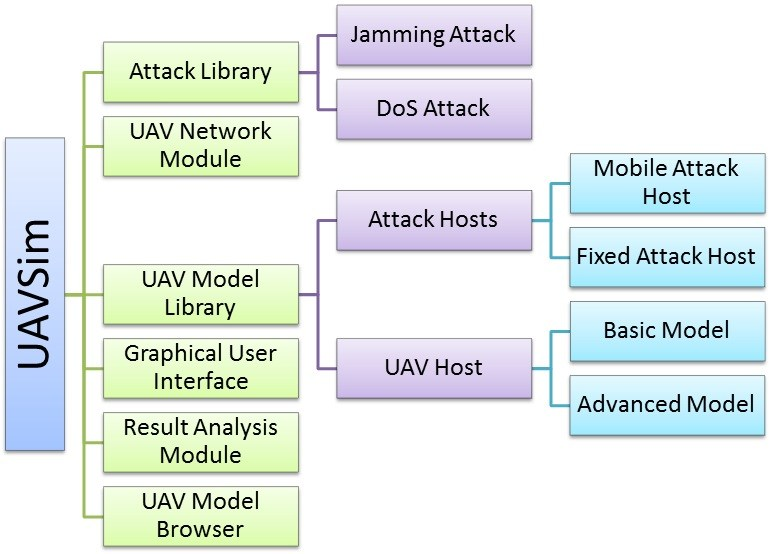
\includegraphics[width = .8\textwidth]{UAVSim1.jpg}  
        \caption{UAVSim架构设计} \label{fig2}
    \end{figure} 
        \subsection{UAV模型库}
        无人机模型库包含所有的无人机模型,以及移动和固定攻击主机模式。基本的无人机模型使用\citep{6javaid2012cyber}\cite{6javaid2012cyber}中给出的架构描绘一架无人机的基本功能。它将无人机描绘为六个组成部分 — — 数据采集模块、 航姿系统 (海拔高度和标题参考系统)、 导航 (导航) 系统、 控制模块、 数据日志记录模块和遥测模块。该模型还可以用于无线攻击主机,基于假设他们有同样的能力。然而,它会浪费的计算资源,目的是在定义模块正在检测和测试的较低层的攻击。这种模型如图\ref{fig3} 所示。应该指出的是,通信模块不会显示在这里,因为它包含所有的子模块。
        \begin{figure}[]
	        \centering          	
            \includegraphics[width = .8\textwidth]{UAVSim3.png}  
            \caption{UAV模块} \label{fig3}
        \end{figure} 
        模型的一些基本属性是允许用户修改的,如无人机速度、 流动性等。高级的用户也将被允许修改默认值和其他参数。所有防御上的对各种攻击将都不得不在 C++ 代码文件中定义。先进的无人机模型允许在通讯时改变相关参数。
        
        \subsection{UAV网络模型}
        本模块定义了UAVNet的各种网络参数,如无线信道、 通信协议和传输范围。类似于其他模块,一些高级的参数不是允许由基本用户更改。在此模块中定义的几个参数,基础无线网络软件包和其他与移动有关的软件包是从 inet 2.0 中导入的。网络在NED文件中定义,仿真需要的库也在NED文件中导入。每个模拟项目有一个配置文件,默认命名为 omnetpp.ini。此文件包含所有的网络参数。在 UAVSim,GUI 可以设置各种参数,用户不需要创建或编辑此文件。高级的用户可以仍然直接编辑此配置文件。
        
        \subsection{攻击库}
        攻击模块包含所有攻击库。它可以帮助设计者考虑对系统的影响,并提高系统的整体安全性。基于 \citep{6javaid2012cyber}\cite{6javaid2012cyber} 中提到的威胁模型,我们选择了两个对无人机影响最大的攻击——DDOS和Jamming. 这些攻击造成巨大威胁,破坏性的损害系统的可用性。
            \subsubsection{DDOS攻击}
            DDoS (分布式 DoS) 攻击旨在网络拥塞,使主机对于其他主机在网络中不可用,大多数情况下,会增加响应时间。我们用多个可被用户定义的攻击节点来实现这种攻击。我们使用传统的向同一个主机发送欺骗报文的方式来启动这种攻击。所有的攻击节点将被分配与常规节点相同的IP段以使他们互相可见。默认的情况下,我们使用30个敌对主机。这个数字是经过作者多次实验校准得来的。
            \subsubsection{干扰攻击}
            干扰攻击需要在任务范围内传输大量噪音,以阻断所有的通讯。这类噪声通常是全频段的,并且会阻断所有的通讯。大多数无线设备无法正确处理这种攻击, 并且这类攻击相对容易进行。这种攻击通过创建NED语言程序,在不同的频率使用轮询机制向所有的节点发射随机信号。
            
        
        \subsection{用户图形界面}
        这是 UAVSim 的最重要组成部分之一。他可以让基础用户简易的更改参数并用特定的参数运行仿真。图\ref{fig4}是它的截图。GUI使测试平台易于使用,并不需要拥有专门的知识。GUI中没显示的参数将被设为默认值。在仿真过程中,会显示实时的网络行为,十分易于视觉化。攻击节点和UAV使用不同的图标表示,帮助用户区分他们。目前,另一个GUI正在开发中,并且其他高级选项需要在配置文件中更改。
        \begin{figure}[]
	        \centering          	
            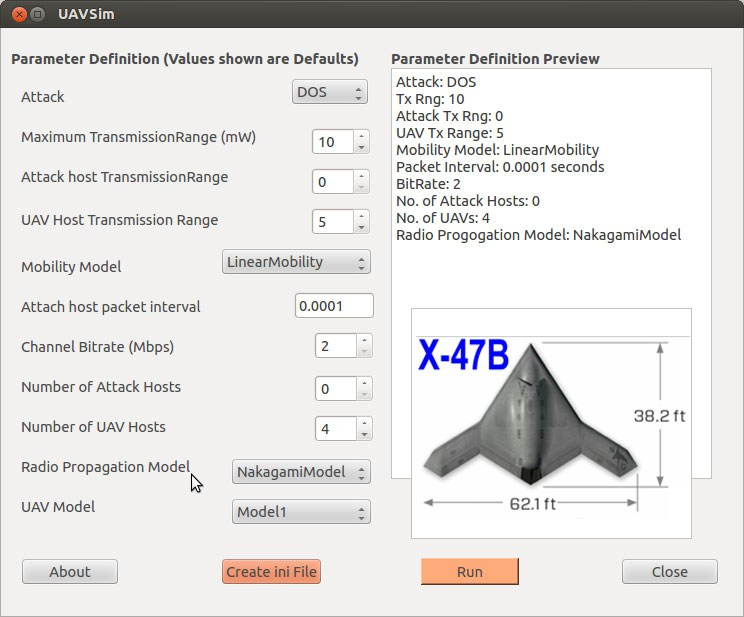
\includegraphics[width = .8\textwidth]{UAVSim2.jpg}  
        \caption{UAVSim简易GUI配置} \label{fig4}
        \end{figure}
        
        \subsection{结果分析模块}
        此模块可以以图形的方式输出各种数据,帮助用户获取信息。结果分析界面计算并显示结果数据,如时间和平均损失。用几次实验积累的数据,该模块可以显示结果图像。
        \subsection{UAV模型浏览器}
        这个模块允许用户使用FlightGear飞行模拟器中的模型。这个模块通过解析XML文档中的参数,将文档转换为模型。不同的工业和研究模型可以通过这个模块简单地生成他们的模型文件并测试。
        
\chapter{攻击分析和结论}
尽管进行了大量的DDOS和干扰攻击分析,但在这里仅对干扰攻击结果进行分析。我们使用测试平台对不同参数的影响进行了分析。在这项工作中,对所有节点间的平局往返时延和丢包率进行了计算,因为这几项数据代表了时间敏感网络的可用性和可靠性。一些默认参数的定义在表\ref{table1}中。
\begin{table}
    \centering
    \caption{无人机网络默认参数}\label{table1}
    \begin{tabular}{@{}ll@{}} \toprule
        参数 & 值 \\ \midrule
        仿真时间限制 & 300秒 \\
        无线电传播模型 & Nakagami模型\cite{22rhattoy2012impact} \\
        UAV发包间隔 & 0.05秒\cite{23zhan2011wireless} \\
        攻击节点发包间隔 & 0.0001秒  \\
        UAV数量 & 10  \\
        攻击节点数量 & 30  \\
        移动模型 & 线性移动  \\
        UAV传输功率 & 5瓦  \\
        攻击节点传输功率 & 10瓦  \\ \bottomrule
  \end{tabular}
\end{table}
    \section{干扰攻击}
    我们使用6个UAV,三个在5GHZ频段上,其他的在10GHZ频段上。每组中的两个节点与第三个阶段通讯。对于干扰攻击,我们评估了对传输距离的影响和攻击节点数量的影响。
        \subsection{传输距离影响}
        攻击主机的传输功率范围是从0到10W不同,而常规的无人机传输功率固定在5W。结果如图\ref{fig5}所示,当攻击机通讯范围增大时攻击机和UAV的丢包率均有所上升,且攻击节点的丢包多于UAV节点。另一个重要的发现是当通讯范围增大,UAV节点的丢包率始终稳定在50%-60%,因此增大攻击节点的传输范围的影响并不如开始攻击造成的影响大
        \begin{figure}[]
	        \centering          	
            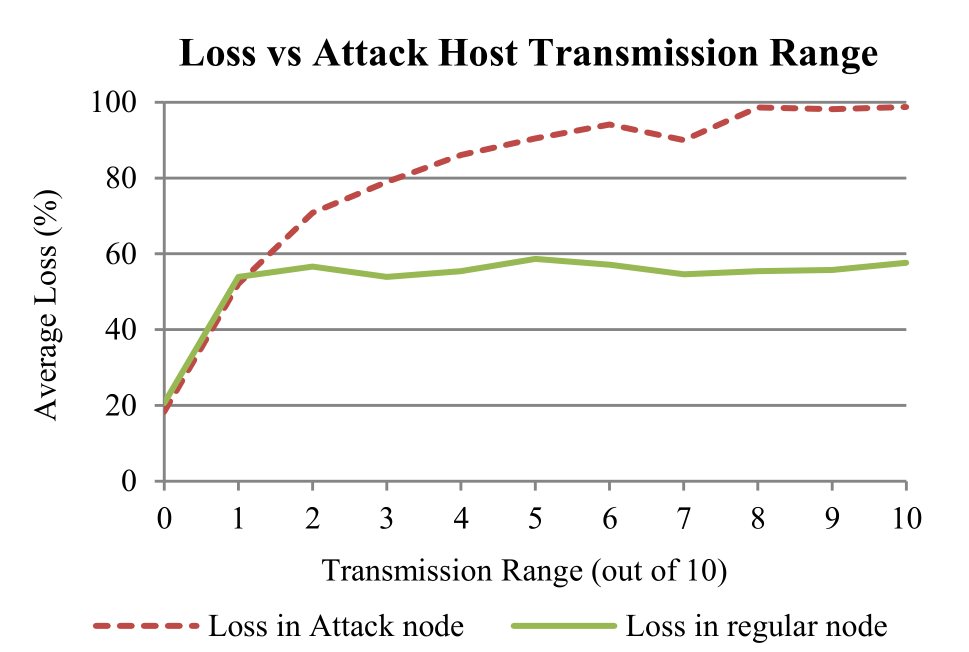
\includegraphics[width = .8\textwidth]{UAVSim4.png}  
        \caption{增大攻击节点通讯范围时网络的整体丢包率} \label{fig5}
        \end{figure}
        \subsection{攻击节点数量影响}
        评估节点数量的影响时,节点传输范围采用定值。我们考虑了如下两个案例,例一,攻击节点的传输范围是10W,普通UAV是5W。例二,攻击节点传输范围是5W,普通UAV是10W。通过对图\ref{fig6},\ref{fig7}的分析,随着攻击节点数量的增长,平均丢包率几乎线性增长,往返时延则几何级数增长。
        \begin{figure}[]
	        \centering          	
            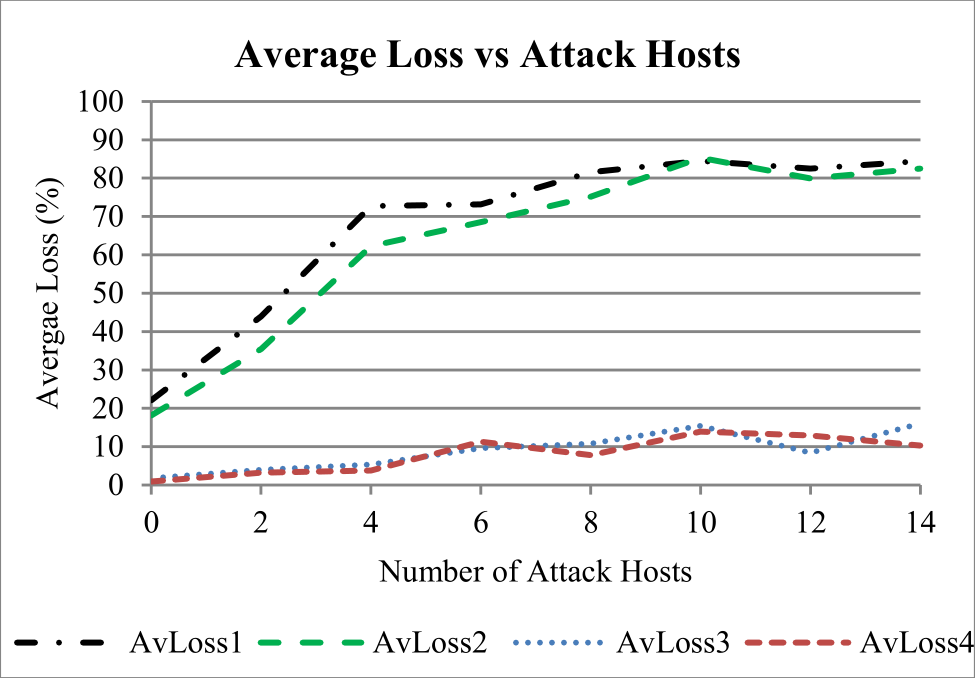
\includegraphics[width = .8\textwidth]{UAVSim5.png}  
        \caption{攻击节点数量增多时网络的整体丢包率} \label{fig6}
        \end{figure}
        \begin{figure}[]
	        \centering          	
            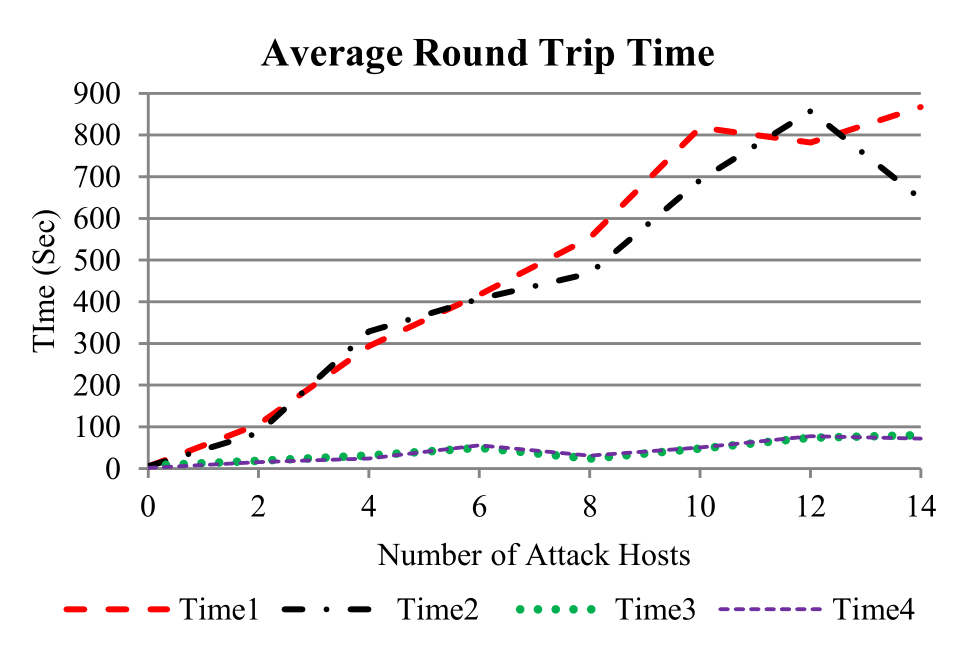
\includegraphics[width = .8\textwidth]{UAVSim6.png}  
        \caption{攻击节点数量增多时网络的平均往返时延} \label{fig7}
        \end{figure}
    \section{分析}
    在本节中,我们讨论从攻击仿真结果图中获得的信息,进一步证明测试平台的能力。
    \begin{itemize}
        \item 在所有模拟中,攻击节点越多,平均丢包率和往返时延也越高。
        \item 启动干扰攻击的攻击节点数量在不同的仿真场景下需是不同的
        \item 随着攻击主机数目的增加,平均数据包丢失呈线性增加,往返时间成倍地增长,从1.6秒到将近14分钟。
        \item 平均丢包在仿真启动前10秒就很快变为99.9%,但在300秒中逐渐下降。这表明,在攻击中,在系统无法工作的前几秒钟,可能需要一些时间才能再次开始通讯。
    \end{itemize}
\chapter{结论和工作展望}
在本文中,我们提出开发无人机网络安全测试平台UAVSim的高效开发方法。UAVSim 允许用户指定不同的无人机模型和不同的攻击,以及用图形的方式产生结果。在UAVSim中仿真了DDos和干扰攻击对无人机网络的影响。通过实验结果印证了UAVSim对无人机网络的仿真能力。也说明这个平台可以用于评估攻击和各种缓解措施。从研究的角度来看,UAVSim是一个模拟攻击对无人机网络影响的新尝试,而且并不只是针对于模拟单一无人机。未来,我们计划在UAVSim中加入新的协议,先进的攻击,和不同的防御手段。

\backmatter                             %% 文后无编号部分
\printbibliography[heading=bibintoc]
\end{document}
